\section{Studying yet another Linear System}\label{sec:p2}

\begin{enumerate}[(a)]
\item 
The system is the linear combination of three states of $x$ (i.e. $n-1, n, n+1$.) Therefore it is linear.

$x[n-1-k]+x[n+1-k]-2x[n-k] = (Lx)[n-k]$. Therefore the system is shift invariant.

The system is defined from both previous and future state of $x$. Therefore it is not causal.

The system depends on the previous state of $x$, i.e. $x[n-1]$. Therefore it is not memoryless.

The impulse response of $x[n-1] + x[n+1] - 2x$ is $3\delta$ (each has impulse response of $\delta$). Since $\delta$ is BIBO stable, the system is BIBO stable.

%----------------------------------------------------------------------------------------------
\item The sketches of $(x_1, Lx_1), (x_2, Lx_2)$, and $(x_3, Lx_3)$ are showed in Figure \ref{fig:p2-1}, \ref{fig:p2-2}, and \ref{fig:p2-3}, respectively.

\begin{figure}[htbp]
	\centering
	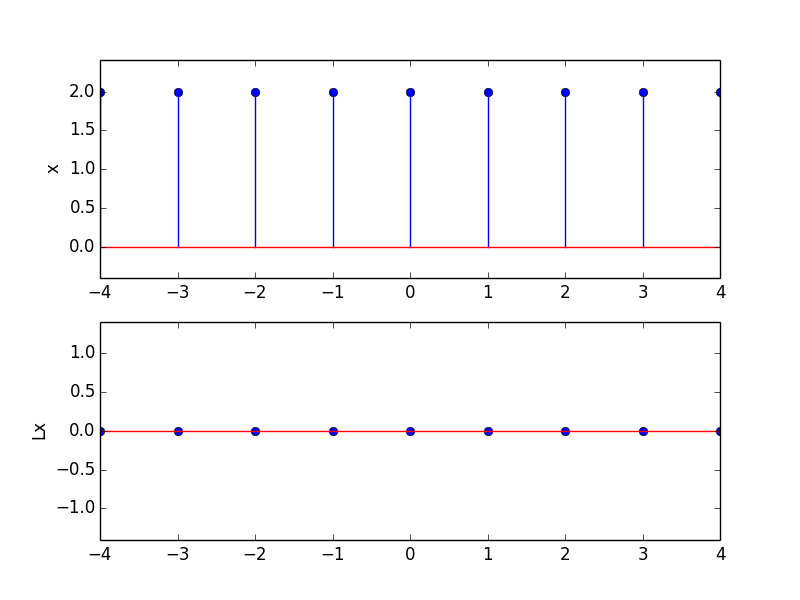
\includegraphics[width=\textwidth,trim={0.2in 0.2in 0.2in 0.2in},clip]{images/p2-1}
	\caption{$x_1$ and $Lx_1$, where  $x_1[n] = c, \forall n \in \mathbb{Z}$. Here $c=2$, but choice of $c$ does not affect $Lx_1$.}
	\label{fig:p2-1}
\end{figure}

\begin{figure}[htbp]
	\centering
	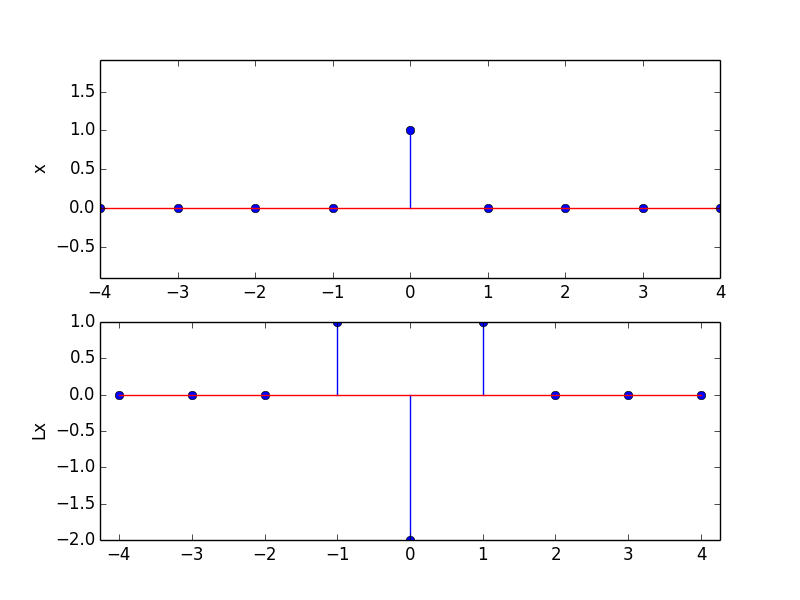
\includegraphics[width=\textwidth,trim={0.2in 0.2in 0.2in 0.2in},clip]{images/p2-2}
	\caption{$x_2$ and $Lx_2$, where $x_2[n] = \delta[n]$.}
	\label{fig:p2-2}
\end{figure}

\begin{figure}[htbp]
	\centering
	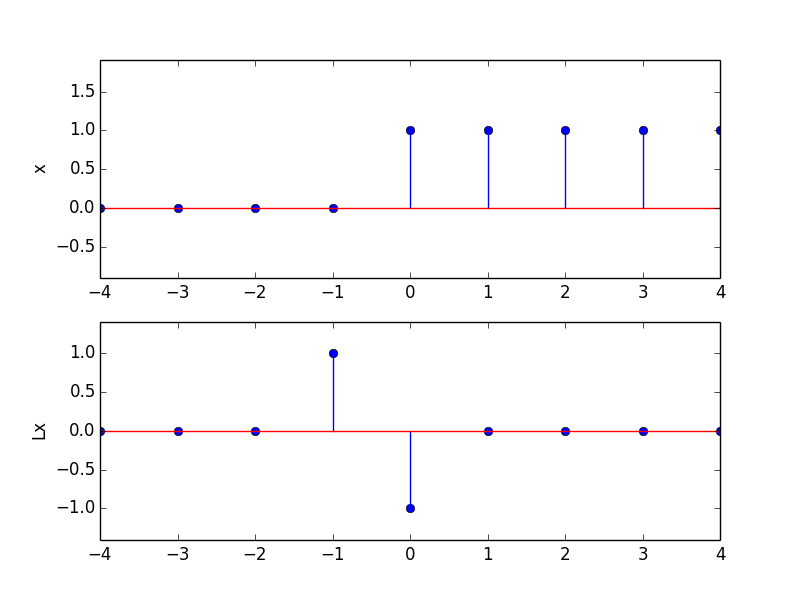
\includegraphics[width=\textwidth,trim={0.2in 0.2in 0.2in 0.2in},clip]{images/p2-3}
	\caption{$x_3$ and $Lx_3$, where $x_3[n] = u[n]$.}
	\label{fig:p2-3}
\end{figure}
\end{enumerate}